This chapter outlines the major nuclear science and engineering theory relevant to spectral shaping and analysis of ETA. 
First, the basic neutron interaction theory that impacts the ability of a source to be shaped into an objective spectrum is discussed. 
Next, the nuclear fission process is outlined with a primary focus on fission product generation. 
After, fundamental aspects of nuclear data and their application in Monte Carlo neutron transport codes and an associated stochastic sampling approach utilizing nuclear data covariance matrices are outlined.
Finally, neutron activation foil theory relevant to the unfolding of a neutron spectrum is examined. 

\section{Neutron Interactions with Matter}
Neutron interaction mechanisms with matter serve as a physical constraint to spectral shaping of a neutron flux spectrum. 
Neutron interactions can act to moderate, absorb, or even emit more neutrons. 
The major reaction mechanisms available in the range of the fast to thermal energies that are relevant to nuclear weapon environments are elastic scattering, inelastic scattering, radiative capture, and the release of `x' neutrons (n,xn) through neutron evaporation.  
% typically (n,x) are a separate subclass of reactions where (n,xn) refers to the family of (n,2n), (n,3n), and so forth reactions
Fission reactions are an extremely important reaction mechanism for the formation of synthetic weapon debris; however, fission does not contribute largely to the spectral modification problem for this application. 
A diagram summarizing the important neutron reactions is shown in Figure \ref{fig:rxns}.

% this is a nice figure.  Being extremely nit-picky - where is elastic scattering?  I put it in there, I guess i thought it was a boring reaction
\begin{figure}[ht]
	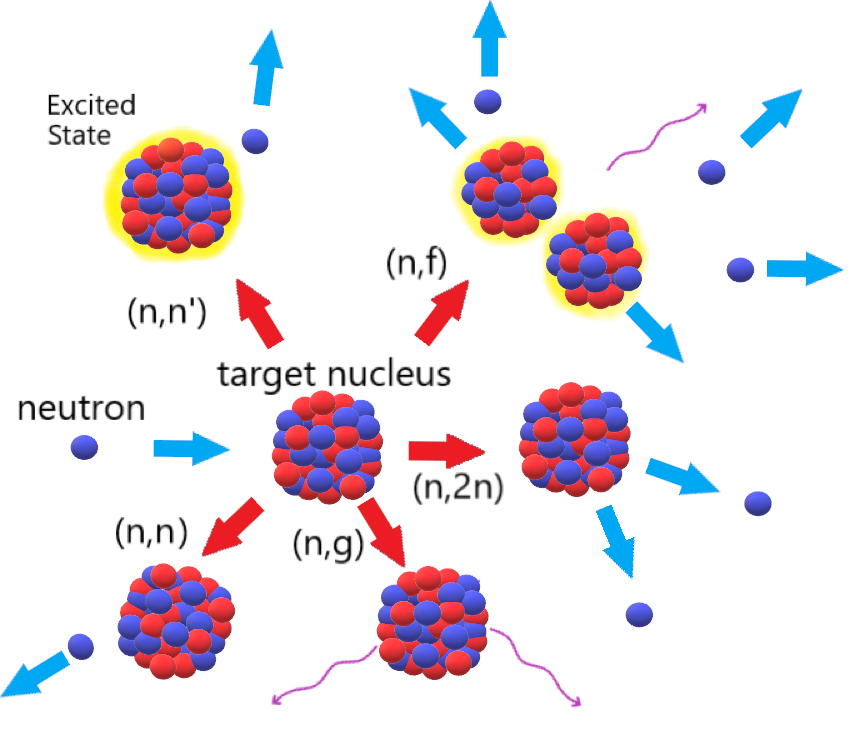
\includegraphics[width=\linewidth]{Figures/Chapter2/NeutronThings.png}
	\caption[Diagram of selected neutron reactions of importance to spectral shaping and fission product generation.]{Diagram of selected neutron reactions of importance to spectral shaping and fission product generation \cite{Greenwood2013}.}
	\label{fig:rxns}
\end{figure}

The neutron interaction probability is described by the neutron microscopic reaction cross-section ($\sigma_{rxn}$), which is a function of the target isotope and incident neutron energy $(E_{n})$.  
The microscopic cross-section multiplied by the atomic number density, $N$, provides the macroscopic cross-section ($\Sigma_{rxn})$, a measure of the interaction probability in bulk material per unit path length traveled. 

% I'd recommend to delete this para.  Sounds good. 
% I don't see where it ties to the following discussion and the fission classification seems a bit early and disconnected.
%Neutrons can be categorized into energy regimes such as thermal, epithermal, and fast, although these regions are relative and vary according to different fields of nuclear sciences or particle physics.  
%A thermal neutron is below 0.025 eV, which is average $E_{n}$, in thermal equilibrium with a 290 K temperature distribution\cite{Duderstadt}. 
%Epithermal neutrons are between 0.025 eV and 1 MeV, and fast neutrons are above 1 MeV.
%In the context of presenting fission product distributions as a function of energy, fast neutrons induce fission under a Watt spectrum at 500 keV, and high energy neutrons are 14 MeV. 

% Need a sentence to preface why the following section is here. As stated, it is unclear what value this para and figure add. I think I'll leave it off to make things condensed. I was going for showing how everything adds up to a total cross-section.  

%The major cross-sections of interest to $^{235}$U up to 20 MeV are displayed in Figure \ref{fig:ntotU}. 
%The total cross-section is the summation of all of the possible reaction mechanisms. 
%Each reaction is explained in further detail below; however, it is important to understand that these reactions are in competition with each other. 
%In general, absorption reactions dominate at low energy. 
%At high energy elastic scattering, inelastic scattering, and (n,xn) reactions are the most probable interaction. 

%\begin{figure}[ht]
%	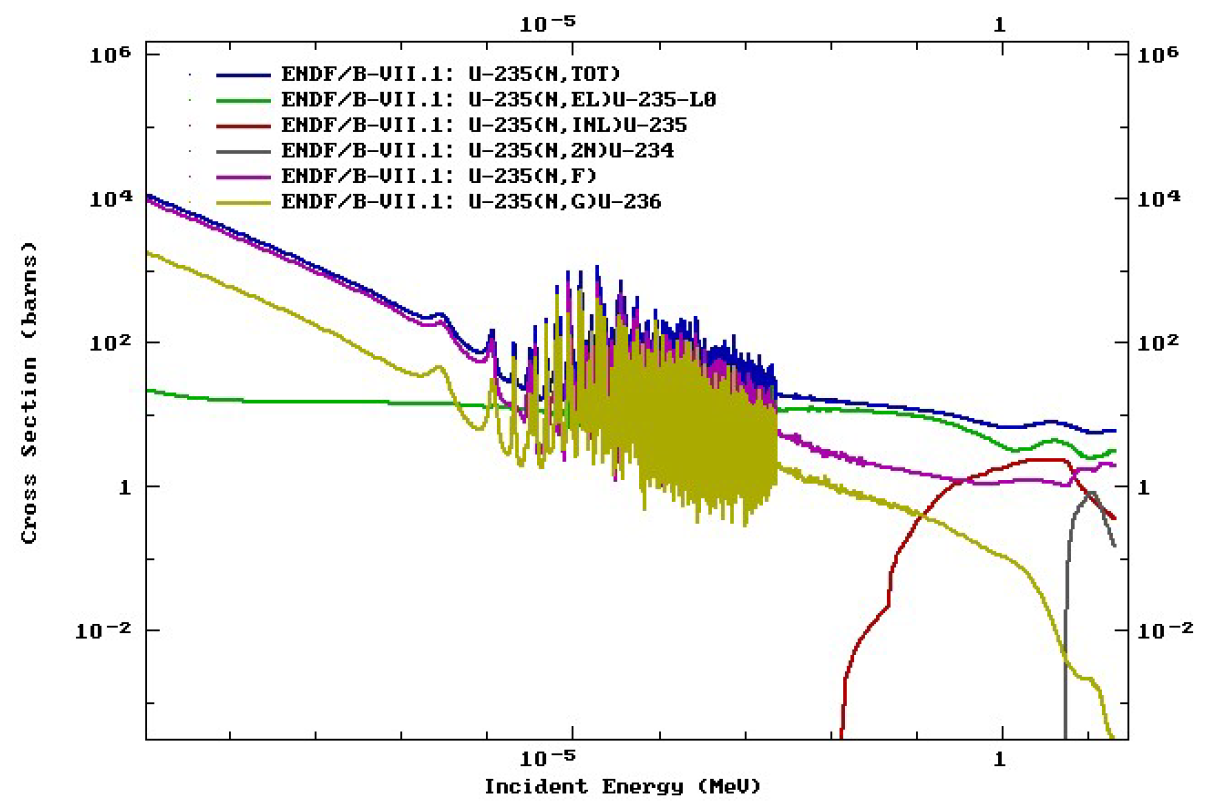
\includegraphics[width=\linewidth]{Figures/Chapter2/n_tot.png}
%	\caption[U-235 (n,f) cross-section compared to competing reaction channels]{U-235 (n,f) cross-section compared to competing reaction channels\cite{ENDF}}
%	\label{fig:ntotU}	
%\end{figure}

\subsection{Elastic Scattering (n,n)}

\ Elastic scattering (n,n) is an extremely important reaction for lowering the average energy of the neutron population by downscattering \cite{Turner}. 
An elastic collision does not place the target nucleus in an excited state, which allows for the simplified use of conservation of energy and momentum to describe the interaction. 
A selected group of elastic scattering cross-sections relevant to the application in the ETA design are shown in Figure \ref{fig:elastic}. 

\begin{figure}[ht]
	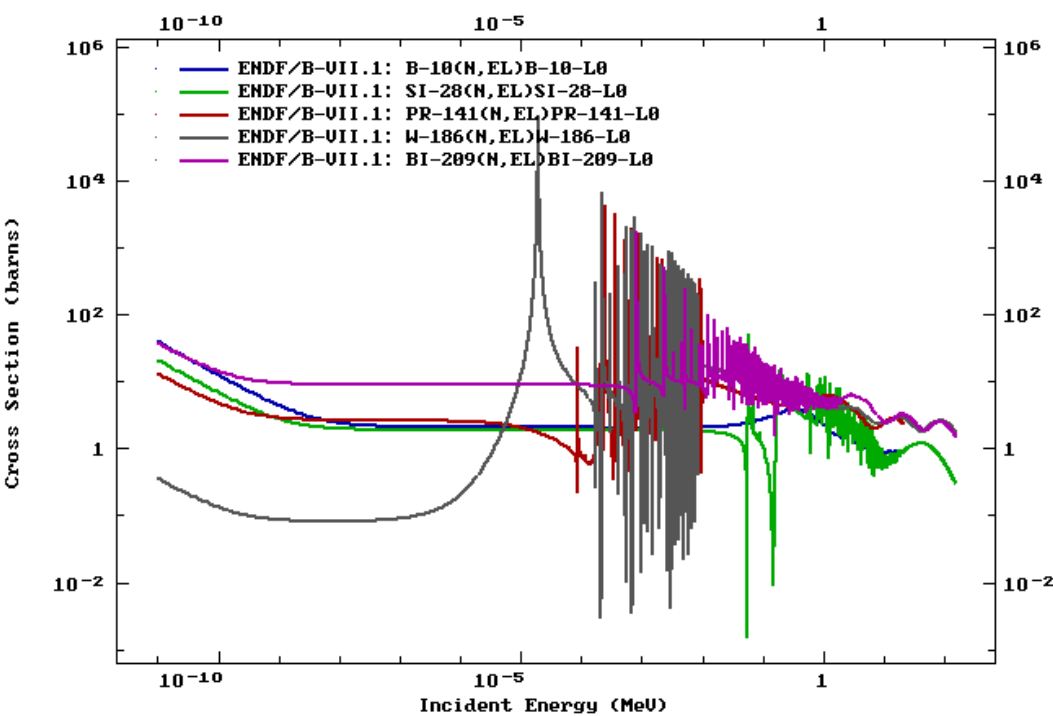
\includegraphics[width=\linewidth]{Figures/Chapter2/elastic.png}
	\caption[Comparison of various elastic scattering cross-sections for materials in the current ETA design]{Comparison of various elastic scattering cross-sections for materials in the current ETA design \cite{ENDF}.}
	\label{fig:elastic}
\end{figure}

\ The maximum energy lost in a neutron elastic collision with a nucleus is a function of the target isotope atomic mass (M). 
Elastic scattering with higher mass isotopes produce a smaller energy loss per collision compared to interactions with low atomic mass nuclei. 
Elastic scattering can transfer nearly all of a neutron's kinetic energy with a collision on hydrogen, while scattering off bismuth will produce very little energy loss. 
The maximum energy transfer (Q) to the target nucleus per collision is given by 

\begin{equation} \label{eq:elastic}
    Q_{max}=\dfrac{4ME_{n}}{(M+1)^{2}}.
\end{equation}
% should define E_n

\subsection{Inelastic Scattering (n,n')}
% This description was a bit off since there are infinite nuclear excited states too (the "continuum". I removed the atomic analogy since it presumed some knowledge about atomic physics; feel free to add back in
\ Inelastic scattering is similar to the reaction dynamics of elastic scattering; however, the target nucleus is placed in an energetically excited state after the impact \cite{Turner}.
The energy of the excited states are governed by quantum mechanics and are unique to particular isotopes. 
An incident neutron, or other particle, can transfer energy to the target nucleus and populate an excited state of the atom.  
For inelastic scattering, this is typically one of the lower discrete energy levels.
However, the incident neutron and target nucleus can form a quasi-continuous spectrum during a compound reaction which gives rise to resonances \cite{Krane}. 
% These resonances have a certain energy width created by states having a energy widths larger than the energy spacing of the states. The width of the resonance is determined by the states. I'm going to delete now. 
% I'm not 100% clear on the last statement 

\ Inelastic scattering is a threshold reaction, meaning an incident neutron must have a minimum amount of energy to enable the reaction channel. 
Additionally, neutrons generally lose more energy per collision with high Z isotopes if the interaction is inelastic compared to elastic scattering. % Is this right? High z tends to have lowere energy states. Changed wording, this is what i meant. 
The energy that would normally be conserved in an elastic collision is reduced in the conservation equations by the energy of the excited state populated. 
Examples of inelastic scattering cross-sections are shown in Figure \ref{fig:inelastic}. %Isotopes from $A=12$ to $209$ are shown to identify the trend of increasing mass number.
% I don't see a trend; I know there is one, but the selected isotopes are all over the place  
% One of them was (g,inl) not (n,inl). fixed 

\begin{figure}[ht]
	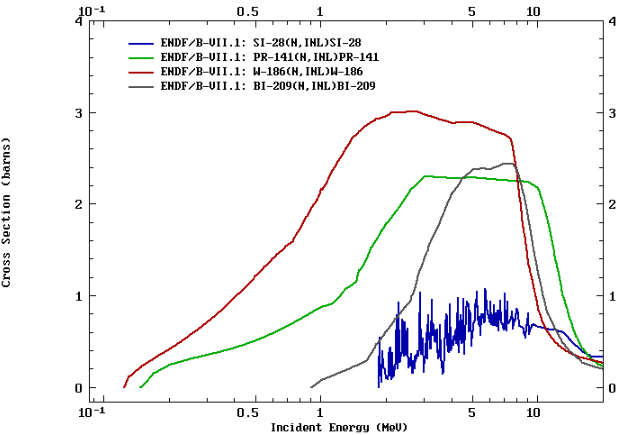
\includegraphics[width=\linewidth]{Figures/Chapter2/inelastic.png}
	\caption[Comparison of various inelastic scattering cross-sections for materials in the current ETA design.]{Comparison of various inelastic scattering cross-sections for materials in the current ETA design \cite{ENDF}.}
	\label{fig:inelastic}
\end{figure}

\ Inelastic scattering is one of the lower threshold energy neutron reactions.
As shown in Figure \ref{fig:inelastic}, there is no general functional form of the threshold energy to enable the reaction by atomic mass. 
The incident neutron threshold energy to cause inelastic scattering with $^{27}$Al, a lighter isotope, is between $^{184}$W and $^{208}$Pb. 
These cross-sections indicate the energy levels of the nuclei itself. 

\ The excited state nucleus can de-excite via gamma emission or other channels if energetically favorable. 
The excited nucleus usually decays in a short time; however, metastable isomeric states can be populated with inelastic scattering and have half-lives on the order of hours or much longer\cite{Krane}. 
These isomeric states have applications in foil activation experiments used for neutron spectrum unfolding, where it may take some time to start measuring the foil activity. 
An energy level and decay mode diagram of $^{115}$In is shown in Figure \ref{fig:In115Rxn}. This isotope is chosen as a representative example because it was used as an activation foil reaction in the modeled ETA results.
The metastable state at 336 keV with spin parity $J^{\pi} = 1/2^{-}$ is important for foil activation experiments for the higher epithermal region.
% Shouldn't this be 115In since that is the (n,n') reaction that you use? Yes, that makes more sense. I think I originally had intended to do something else with this. 

\begin{figure}[ht]
	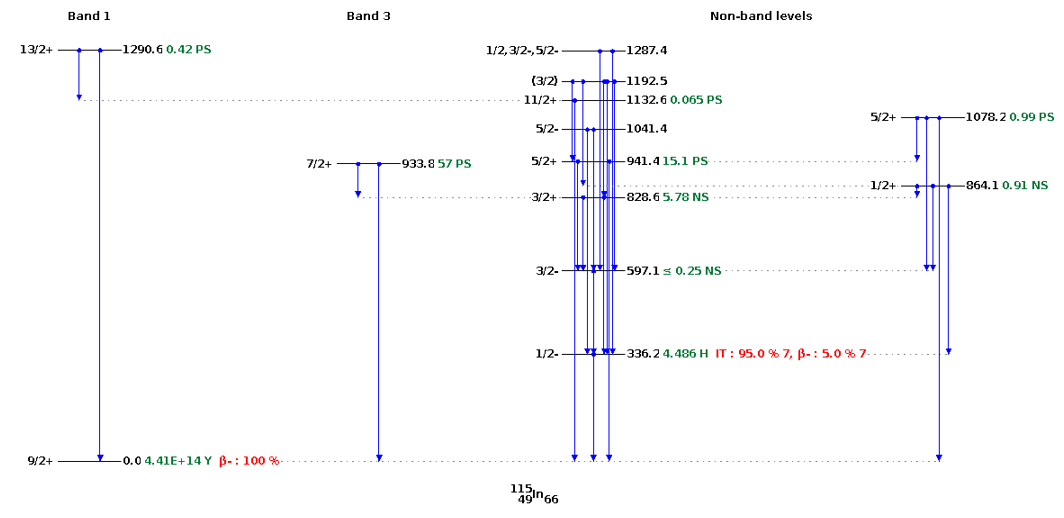
\includegraphics[width=\linewidth]{Figures/Chapter2/TruncatedIn115.png}
	\caption[$\mathrm{^{115}}$In energy level and decay mode diagram truncated at 1.3 MeV.]{$\mathbf{^{115}}$In energy level and decay mode diagram truncated at 1.3 MeV. Plots produced using the Online Service retrieval code package written by C. L. Dunford, National Nuclear Data Center, Brookhaven National Laboratory.}
	\label{fig:In115Rxn}
\end{figure}

\subsection{Neutron Evaporation (n,xn)}

\ A neutron can interact with a nucleus and eject additional neutrons. 
The (n,xn) reactions such as (n,2n) and (n,3n) require a threshold energy to separate the neutron from the original nucleus, appropriately called the neutron separation energy. 
Neutron separation energies are on the order of a few MeV to tens of MeV \cite{Krane,n2ns}. 
Increasing the incident neutron energy allows for the evaporation of more neutrons from the nucleus. 

\ The (n,xn) mechanism can occur as a direct reaction, where the incident neutron interacts with only a few particles in the nucleus, or as a compound reaction, where the incident neutron interact with the entire nucleus and is absorbed \cite{Turner}. 
Example (n,2n) reactions are shown in Figure \ref{fig:n2n}. 
The cross-section threshold is generally lower for higher atomic mass isotopes, which have neutrons that are not as tightly bound to the nucleus. 

\begin{figure}[ht]
	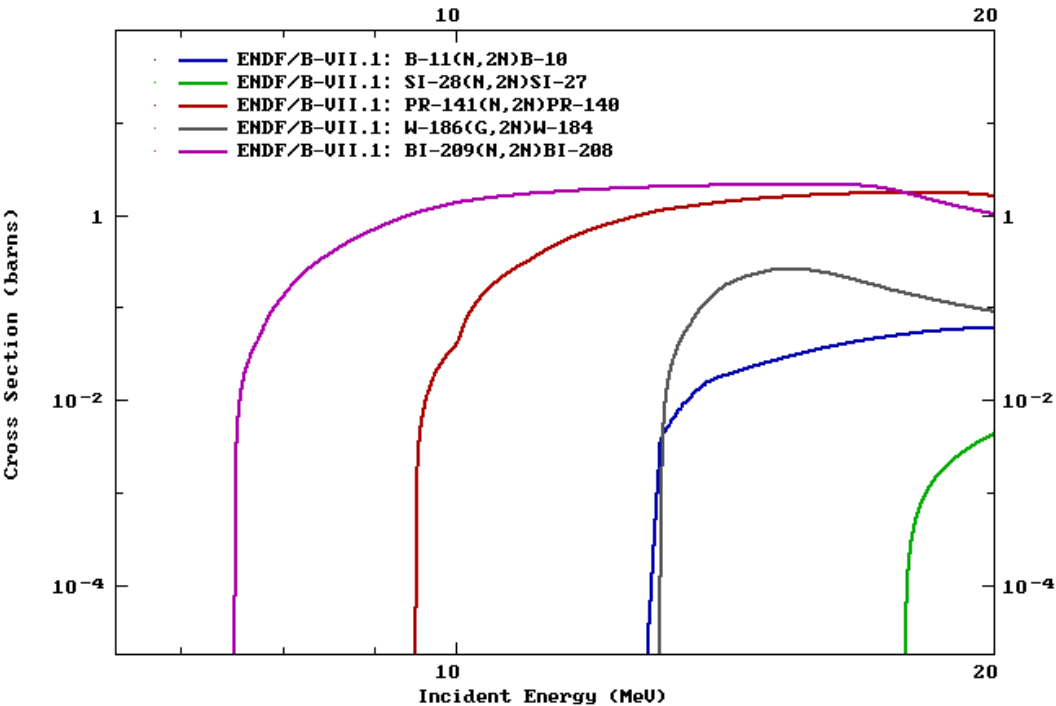
\includegraphics[width=\linewidth]{Figures/Chapter2/n2n.png}
	\caption[Comparison of various (n,2n) cross-sections for materials in the current ETA.]{Comparison of various (n,2n) cross-sections for materials in the current ETA\cite{ENDF}.}
	\label{fig:n2n}
\end{figure}

\ In the context of spectral shaping, (n,xn) reactions are significant for two reasons. 
First, the interaction increases the total neutron population by sacrificing a high energy neutron. 
Second, the neutron energies are lower post-reaction because the reaction is required to overcome the potential barrier and losses through gamma emission. 
% It turns out, for compound rxs, that the emitted neutrons are have a Watt (evaporative) energy distribution 
The lowered neutron energy is beneficial for building up lower energy neutron populations. 
Additionally, this reaction mechanism has applications in foil activation experiments for determining the high energy neutron population.  

\subsection{Radiative Capture (n,$\gamma$)}

Radiative capture, labeled (n,g) and (n,$\gamma$) in literature, is a reaction mechanism most prominent at low energies where an incident neutron is absorbed into the nucleus and a gamma-ray is emitted \cite{Krane}. 
At low energies (below approximately 1 keV, isotope dependent) the absorption cross-section follows the ``1/v" law, so the probability increases with the inverse of the square of $E_{n}$ \cite{Turner}. 
Figure \ref{fig:ngamma} provides examples of selected (n,$\gamma$) cross-sections. 

\begin{figure}[ht]
	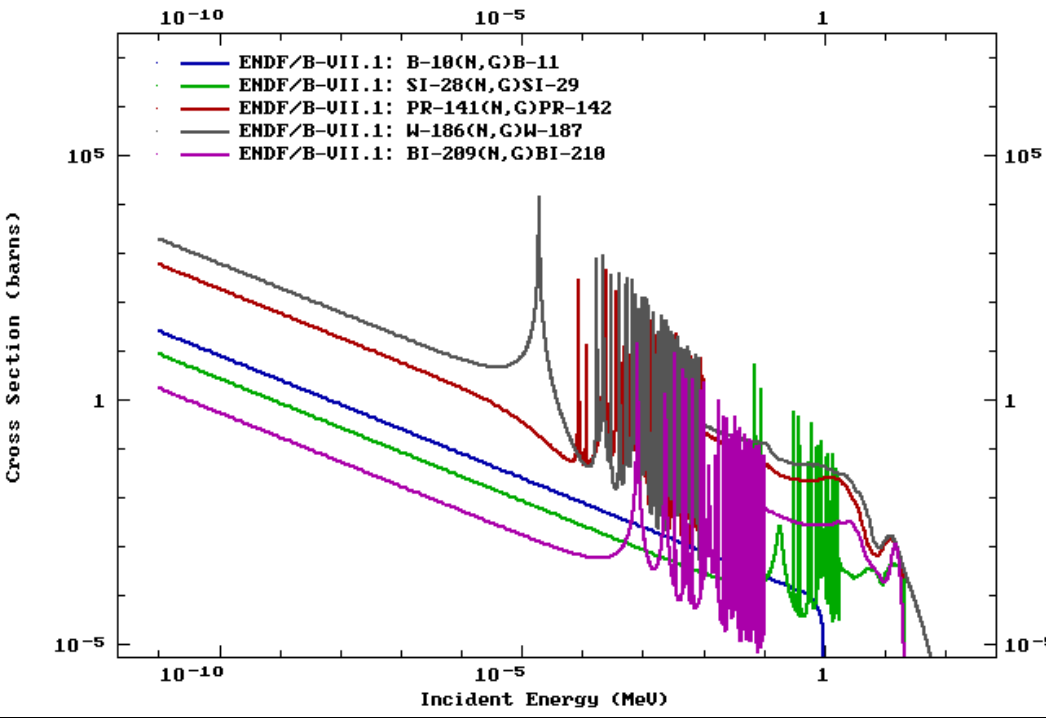
\includegraphics[width=\linewidth]{Figures/Chapter2/ngamma.png}
	\caption[Comparison of various (n,$\gamma$) cross-sections for materials in the current ETA.]{Comparison of various (n,$\gamma$) cross-sections for materials in the current ETA \cite{ENDF}.}
	\label{fig:ngamma}	
\end{figure}

\ Radiative capture is an important absorption reaction mechanism in a few ways. 
The (n,$\gamma$) reactions are of interest to foil activation experiments, specifically for determining the thermal spectrum. 
The resonance structure of the cross-section in the epithermal region can also be used to generate a unique response. 
Radiative capture is generally undesirable for spectral shaping, acting as a poison to the neutron economy. 
Fortunately, the 14 MeV NIF source, is not largely impacted by radiative capture until the neutrons have been moderated, but the ($n,\gamma$) reaction can be used to absorb excess thermal neutrons \cite{Bevins, Krane}. 

\section{Nuclear Fission}
\subsection{Fission Theory}
\ In nuclear fission an excited nucleus breaks up into two or more fission fragments. 
Fission releases a large amount of energy, which is distributed as kinetic energy in the fission fragments, neutrons, gamma-rays, and delayed decay energy. 
The amount of energy liberated is dependent on the specific reaction products and incident neutron energy, so an average number  (approximately 200 MeV) is usually given.
The delayed decay energy is associated with the decay of the unstable fission products, which includes energy in the form of beta ($\beta$) particles, additional gamma-rays, anti-neutrinos, and neutrons. 
A schematic of the fission process is shown in Figure \ref{fig:fission}.

\begin{figure}[ht]
	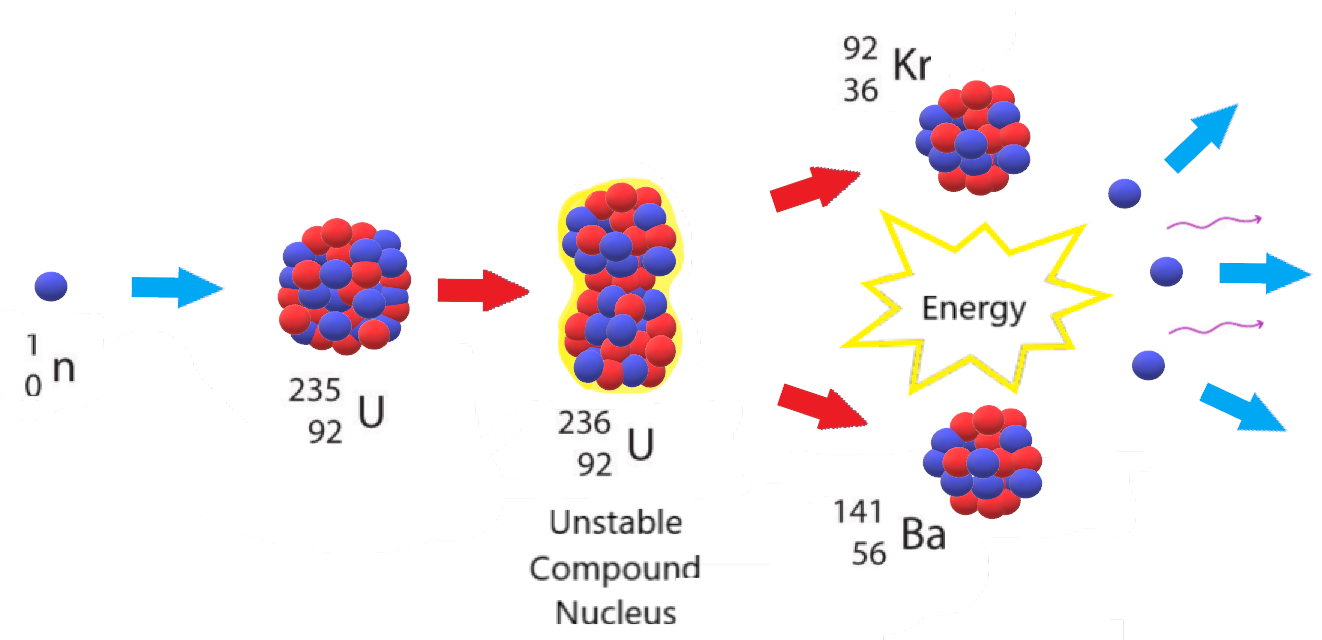
\includegraphics[width=\linewidth]{Figures/Chapter2/Fission.png}
	\caption{Schematic overview of $^{235}$U neutron induced fission. }
	\label{fig:fission}	
\end{figure}

Fission occurs most often in high atomic mass nuclei, such as $^{235}$U, $^{238}$U, or $^{239}$Pu; however, any isotope can be fissioned at large enough incident energies. 
The fissioned isotope separates into two or occasionally three nuclei\cite{Bridgman}. 
Fissionable isotopes like $^{238}$U, $^{240}$Pu, $^{242}$Pu have a significant fission barrier and are incapable of sustaining a nuclear chain reaction. 
Fissile isotopes like $^{235}$U and $^{239}$Pu are capable of sustaining a nuclear chain reaction and have cross-sections with similar characteristics to the radiative capture cross-section shown in Figure \ref{fig:ngamma}. 

The unstable compound nucleus can be modeled at high excitation energies, well above the fission barrier, as an incompressible liquid drop\cite{Krane,Tonchev0}. 
The deformation of the nucleus causes increased surface energies, which are balanced with the Coulomb force (charge repulsion), the strong  nuclear force, and shell pairing effects. 
The perturbation creates an increase in the surface energy and decrease in the Coulomb repulsion because the charge is spread out\cite{Randrup2012}. 
During the fission process, the evolving compound nucleus can emit pre-fission neutrons, known as multi-chance fission \cite{Randrup2012}. 
First-chance fission is the emission of no neutrons, second-chance fission is the emission of one neutron, and so on.  
Multi-chance fission is of particular importance to the mass chains observed in the fission product distribution.

Immediately following the fission event, the fission fragments are in a highly excited state.
Fission fragments are generally very neutron rich compared to the valley of stability. 
The excited fragments emit photons to de-excite and may have enough energy to evaporate more neutrons \cite{Randrup2012}. 
The prompt fission product yield is the distribution of products post neutron evaporation from the fission fragments.  
The fission process releases 2-3 neutrons on average, and this average increases with incident neutron energy due to multi-chance fission and an increase in fission fragment excitation energy. 

\subsection{Fission Products}

The fission product distribution of thermally induced fission tends to be centered around isotopes with closed nuclear shells. 
These isotopes  have a ``magic number" of protons and neutrons, similar to the filled electron structure of the noble gases. 
The fission fragment distribution from thermal neutrons incident on $^{235}$U is shown in Figure \ref{fig:GEF_U}. 

\begin{figure}[htb!]
	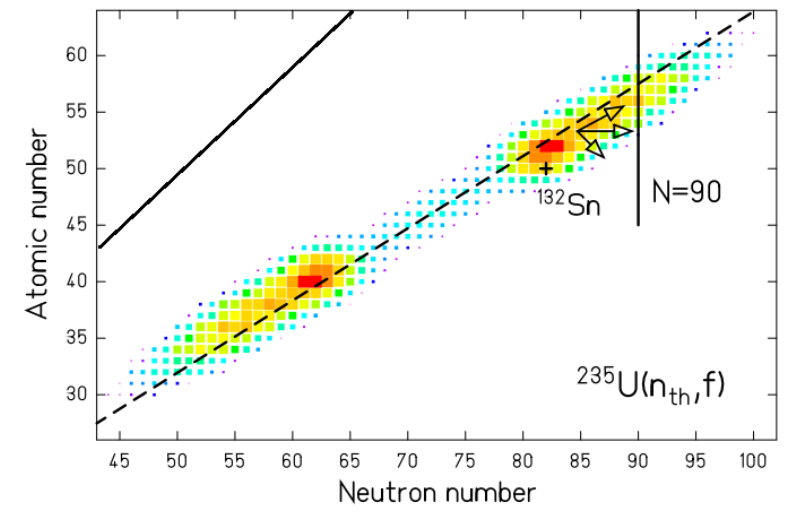
\includegraphics[width=\linewidth]{Figures/Chapter2/U_235Band.png}
	\caption[GEF calculated $\mathrm{^{235}}$U thermal fission product distribution prior to prompt neutron emission.]{GEF calculated $\mathbf{^{235}}$U thermal fission product distribution prior to prompt neutron emission. The dashed line is the neutron to proton ratio of $\mathbf{^{235}}$U prompt fission products and the solid line in the upper left is a ratio of 1\cite{Schmidt2014}.}
	\label{fig:GEF_U}	
\end{figure}

Low-Z stable nuclei have approximately equal numbers of protons and neutrons, but larger nuclei require more neutrons to mitigate the Coulomb repulsion of protons \cite{Krane}. 
Most of the decay products following fission are beta emitters, which occurs because the products are neutron-rich and become more stable upon the conversion of a neutron to a proton. 
Figure \ref{fig:DMode} shows the primary decay modes of isotopes as they decay to the valley of stability. 
In the region of fission products, the primary competing decay mode to $\beta{-}$ is neutron emission, resulting in cross-mass chain transfers after the initial fission process. 

\begin{figure}[htb!]
	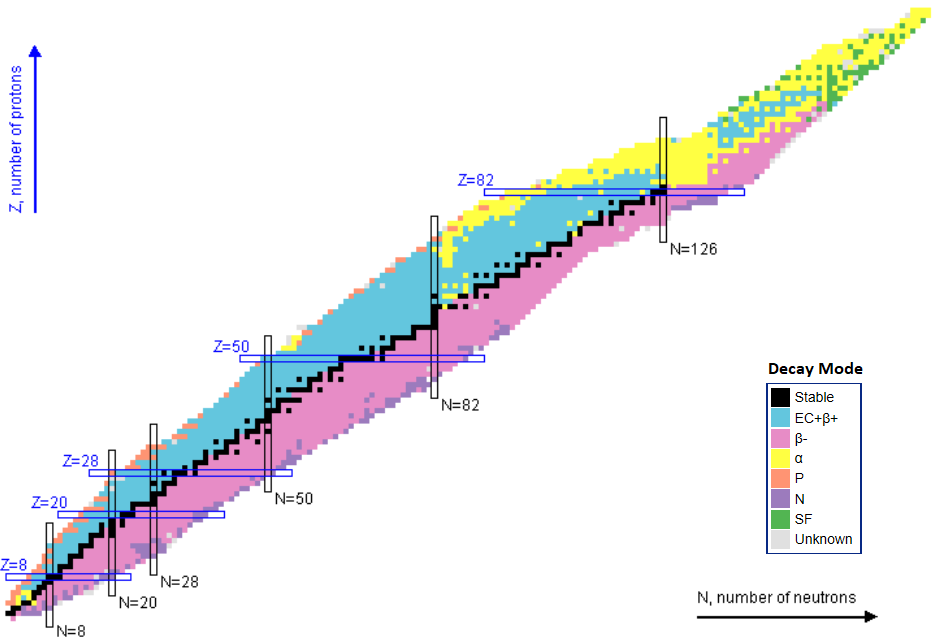
\includegraphics[width=\linewidth]{Figures/Chapter2/DecayModes.png}
	\caption[Primary decay modes of isotopes.]{Primary decay modes of isotopes. Plots produced using the Online Service retrieval code package written by C. L. Dunford, National Nuclear Data Center, Brookhaven National Laboratory.}
	\label{fig:DMode}
\end{figure}

Fission yields can be described by the independent, cumulative, and chain yields. 
The independent yield, $Y_{ind}$, is the prompt fission product distribution directly after the fission event before successive decay \cite{Nichols2008}.
$Y_{ind}$ for $^{235}$U thermal fission is shown in Figure \ref{fig:indy}.
The independent isomeric yield is defined as \cite{indy}

\begin{equation} \label{eq:Indy}
Y_{ind}(A,Z,I) = Y(A) \ \ f(A,Z) \ \ R(A,Z,I), 
\end{equation}

\noindent where the sum yield ($Y(A)$) is the sum of all independent fission products for a given mass A, the isomeric yield ratio ($R(A,Z,I)$) is the the production of each isomer ($I$) for a given independent yield, and the the fractional independent yield ($f(A,Z)$) defines the yield of a particular isotope. 

\begin{figure}[htb!]
	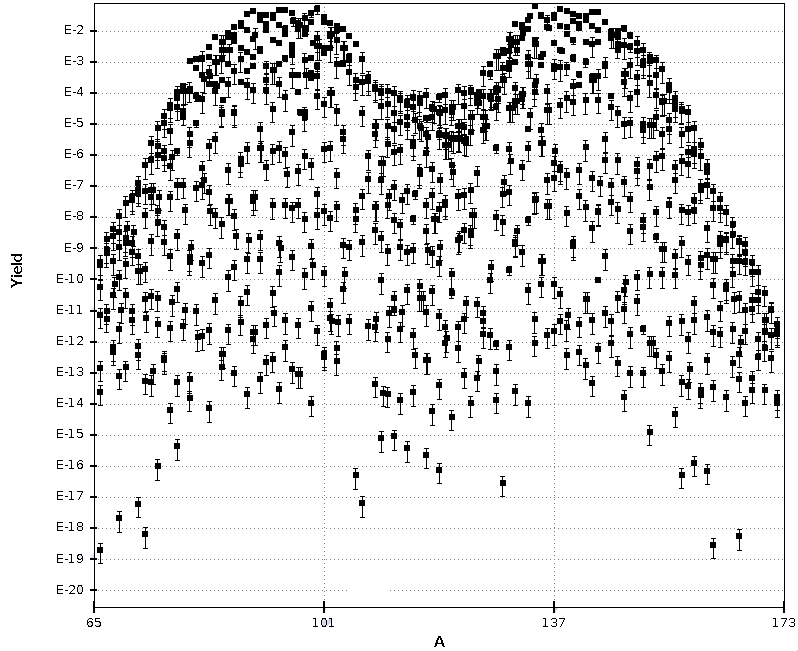
\includegraphics[width=\linewidth]{Figures/Chapter2/indfy.png}
	\caption[Independent fission product yield of thermal fission of $\mathrm{^{235}}$U]{Independent fission product yield of thermal fission of $\mathbf{^{235}}$U. Plots produced using the Online Service retrieval code package written by C. L. Dunford, National Nuclear Data Center, Brookhaven National Laboratory.}
	\label{fig:indy}
\end{figure}

The independent yield produces a cascade of decay chains leading to the cumulative yield, $Y_{c}(A,Z,I)$. $Y_{c}$ represents the production of an isotope over all time after all prompt and delayed emissions and decays. $Y_{c}$ is normally the quantity that is measured in experiments. The cumulative yield is given as \cite{Privas2016}

\begin{equation} \label{eq:Cumulative}
Y_{c}(A,Z,I) = Y_{ind}(A,Z,I) + \sum_{j=0}^N Y_{c}(A_{j},Z_{j},I_{j}) \; b_{j}.
\end{equation}

\noindent where $b_{j}$ represents the branching ratio from isotope $j$ into the cumulative yield and $N$ defines the total number of decay channels into the cumulative yield isotope. 
The cumulative yields for thermal, fast, and high energy fission of $^{235}$U are shown in Figure \ref{fig:U235Cumulative}. 

\begin{figure}[htb!]
	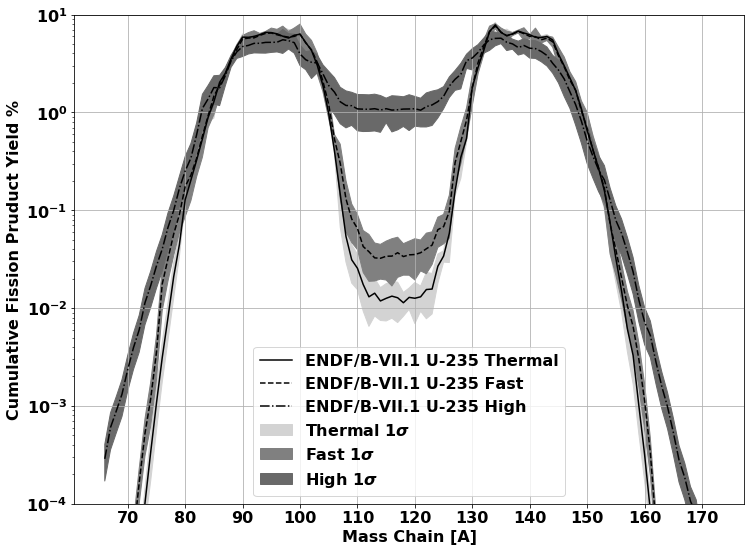
\includegraphics[width=\linewidth]{Figures/Chapter2/ENDF_FPs.png}
	\caption[Comparison of energy dependent${^{235}}$U cumulative fission product distributions]{Comparison of energy dependent $\mathbf{^{235}}$U cumulative fission product distributions from ENDF/B-VII.1 \cite{ENDF}.}
	\label{fig:U235Cumulative}	
\end{figure}

% This makes way more sense with Walid's lecture notes. I am leaving out sum chains, because they are not used. - glad they helped!
As shown in Figure \ref{fig:U235Cumulative}, fission product yields are dependent on the energy of the incident neutron and the identity of the fissioning nucleus. 
The fission products populate one heavy and one light peak. 
The region between the peaks is referred to in this work as the valley, and the low population tails falling off either peak are the wings. 
As the energy of the incident neutron is increased, the valley and wings of the fission product distribution are raised because the fission process becomes more symmetric \cite{Tonchev0}. 
The uncertainty in the fission product yields varies significantly; the fast fission relative uncertainty ranges from 1.6\% for mass chain 137 to 64\% for mass chain 109 \cite{ENDF}. The uncertainty for each fission product is representated at the 1$\sigma$ level as bands in Figure \ref{fig:U235Cumulative}.

\ Finally, the chain yield for a particular mass chain is defined as the sum of the cumulative yields to the final decay to a stable isotope in that mass chain \cite{Nichols2008}. 
The chain yield leads to the cumulative distribution accounting for branching in and out of a mass chain through neutron emission.
In particular, the chain yield equals the cumulative yield for the last stable member of a decay chain.  
An example is shown in Figure \ref{fig:89} for the A = 89 mass chain, where the stable isotope is Y-89\cite{SINGH20131}. 
The neutron deficient decay scheme has not been shown as it has negligible contribution to the fission product decay scheme. 

\begin{figure}[htb!]
	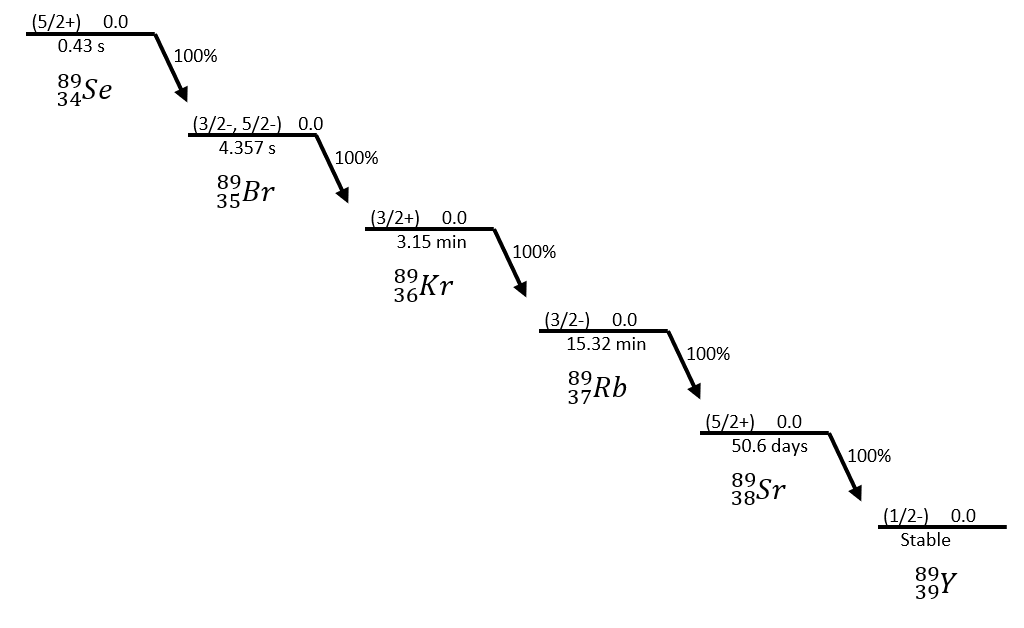
\includegraphics[width=\linewidth]{Figures/Chapter2/89MassChain.png}
	\caption[Simplified neutron rich decay scheme for mass chain A=89. The $\mathrm{^{89}}$Sr decay to $\mathrm{^{89}}$Y represents the final decay to the stable isotope.]{Simplified neutron rich decay scheme for mass chain A=89. The $\mathbf{^{89}}$Sr decay to $\mathbf{^{89}}$Y represents the final decay to the stable isotope \cite{SINGH20131}.}
		\label{fig:89}	
\end{figure}

%The radioactive emissions of the final decay can be used to measure the cumulative fission product yield for an isotope. 
%Some mass chains are more well-behaved for measuring the cumulative yield. For example, the $A=89$ mass chain has many decays that have very short half-lives, up to the precursor stage for the stable isotope. 

% This feels like this should be in Ch1 and is a bit out of place here. Rolling from the disscusion of FPs into how to predict the yield flows better IMO. Moved to Intro

\subsection{Nagy Fits for Fission Product Isotopes}

% I would add a transition sentence to tie the three formalized fissioning energies shown in Fig 12 to this section and motivate why fitting empirical data is needed or makes sense.
The three fissioning isotope energies provided in ENDF describe part of the behavior of the fissioning system as a function of neutron energy.
However, including fits to experimental data enables better energy resolution and predictions consistent that are consistent with observed experiments.  
Empirical relations developed by Nagy, \textit{et al.} provide an approach to predict the fission product yield as a function of energy given sufficient yield measurement data \cite{Nagy1978}.
Nagy fits the fission product experimental data to an exponential equation 

\begin{equation} \label{eq:nagy}
Y(E_{n}) = Y_{0}e^{bE_{n}}.
\end{equation}
where the fitting parameters $b$ and $Y_{0}$ represent the slope of the function in logarithmic form and thermal fission yield, respectively\cite{Nagy1978}. 
The slope is the primary measure of the energy dependency of the fission product yield, which requires  modifications for multi-chance fission.
First chance fission is dominant from up to 5.5 MeV, and second-chance fission up to 14.1 MeV\cite{Nagy1978}. 
Multi-chance fission effects on the fission product yield are less pronounced in asymmetric regions but can have a large impact in symmetric fission ($109 \leq A \leq 129$)\cite{Bevins}\cite{Nagy1978}. 

It is important to note that data-based phenomenological models are not perfect predictors of determining fission products \textit{a priori}. 
In particular, recent publications have findings that cannot be accurately modeled with current theoretical approaches \cite{Tonchev0}. 
In general, there are large uncertainties in the predictive power of calculating energy dependent fission product yields. 
Still, this type of empirical fit has lower predicted error than GEF for individual isotopes where sufficient energy-dependent measurements exist. 

\section{Nuclear Data}
\subsection{Nuclear Data Libraries}

\ Nuclear data relevant to neutrons has been collected for the better part of the last century. 
Nuclear data available for modeling and simulations is collected and published in evaluated data files. 
% Technically the experimental data is published in EXFOR, which the evaluators use to generate the evaluated data files.
There are many versions of evaluated nuclear data, which all aim to characterize the relevant physics backed by experimental results. 
For example, the primary U.S.-based nuclear data file is the Evaluated Nuclear Data File (ENDF). 
Other nations or organizations also have independent evaluations of the available nuclear data. 
Examples of other nuclear data libraries are the Russian National Library of Nuclear Data (ROSFOND), the European Joint Evaluated Fission and Fusion (JEFF) Nuclear Data Library, Japanese Evaluated Nuclear Data Library (JENDL), Chinese Evaluated Nuclear Data Library (CENDL), and the International Reactor Dosimetry and Fusion File (IRDFF).

Figure \ref{fig:RxnComp} shows the evaluation of $^{197}$Au (n,2n) reaction for various libraries. 
In some cases, the library evaluation can be drastically different. 
However, sometimes the libraries are drawing from the same data and models, which can be noted by the overlapping evaluations. 

\begin{figure}[ht]
	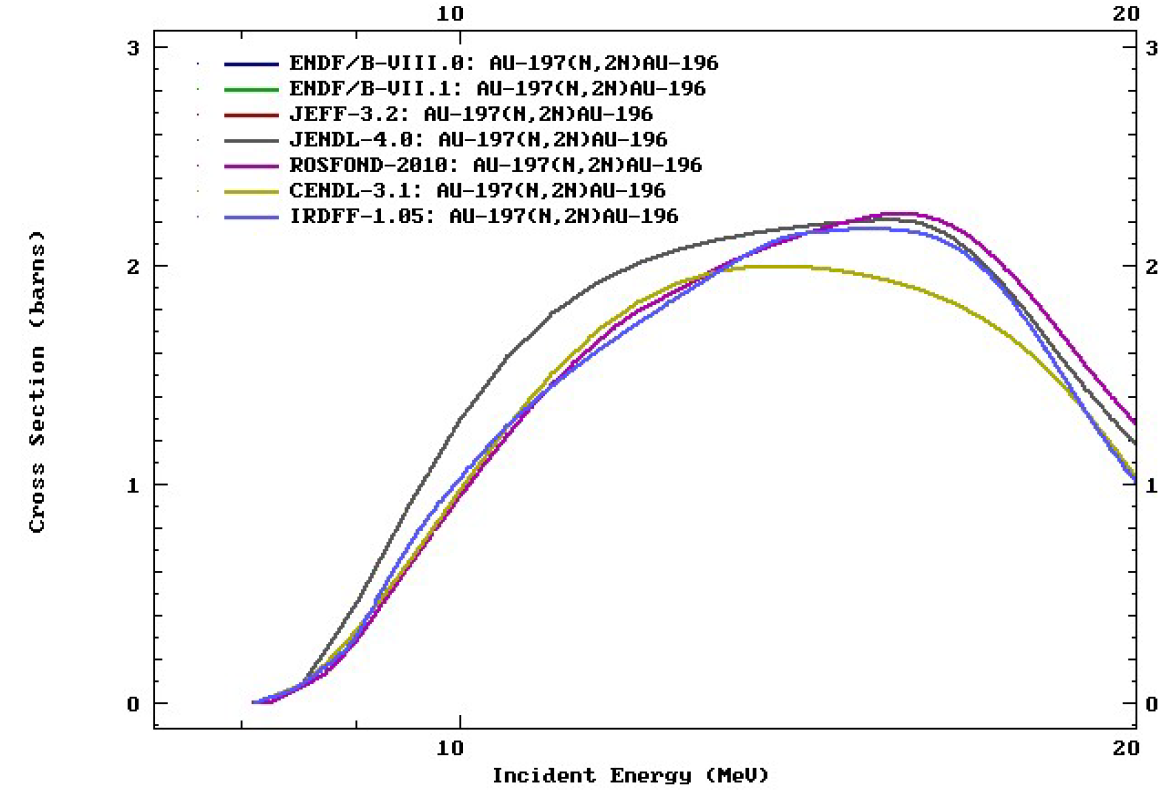
\includegraphics[width=\linewidth]{Figures/Chapter2/RxnComp.png}
	\caption[Comparison of various library evaluations of the  $^{197}$Au (n,2n) cross-section.]{Comparison of various library evaluations of the $\mathbf{^{197}}$Au (n,2n) cross-section \cite{ENDF}.}
	\label{fig:RxnComp}
\end{figure}

\ The experimental data that feeds into ENDF is contained in EXchange FORmat (EXFOR), where the experiment uncertainty, if available, is tracked.
Nuclear data evaluators need reaction models to fill in the gaps where experimental data does not exist.  For example, experiments with sub-electron-volt neutron energy resolution are not feasible at the present time. 
ENDF relies on evaluations of EXFOR data based on experimental quality, statistics, and theoretical basis to fill in areas lacking experimental data \cite{Brown2015}. 
ENDF then stores the underlying nuclear data (cross-sections, angular distributions, half-lives, ect.) that can be used in simulations. 

\ Benchmarking the evaluated nuclear data is done primarily through testing integral results, such as the effective neutron gain-to-loss ratio ($k_{eff}$) of a critical assembly \cite{Brown2015}. These integral measurements provide a more accessible measurement that can be done with high precision and accuracy, as precise as a relative error of 0.01\%, to validate microscopic cross-sections. The use of integral benchmark experiments is important for comparing the net result of the nuclear data; however, there are uncertainties and correlations in the independent reactions that combine to create the integral results. 

\ Validation experiments, applications, studies, and integral benchmarks performed increase the base and accuracy of the nuclear data\cite{Brown2015}.
However, it is important to note that the experiments used to measure nuclear data may have uncertainties that vary by orders of magnitude. An interesting feature of this fact is that the relative nuclear data uncertainty does not always decrease between successive library versions. One example is the increase in uncertainty in the neutrons released per thermal fission of $^{235}$U, which increased from 0.311\% to 0.385\% between ENDF/B-VII.0 to VII.1 \cite{Bostelmann2017}. Another example demonstrating the nuclear data uncertainty is that evaluated $\mathrm{^{6}}$He half-life has changed by approximately 5\% with large increases in the relative error over the last 50 years\cite{he6}.

\  Another prevalent issue is that the majority of accurate measurements were performed for nuclear reactor studies, which limits accessibility to reliable data in different energy domains. As a consequence of this, ENDF only contains fission production data at thermal, fast (0.5 MeV), and high energy (14 MeV). To combat this challenge, smaller, more application-specific libraries have been developed. 

\ The International Atomic Energy Agency (IAEA) provides data to the benchmarked neutron dosimetry reaction IRDFF library \cite{IRDFF}. This library is noted because it is used in the PNNL STAYSL code system, discussed in Section \ref{STAYSLthing}. The IRDFF v.1.05 library contains ``state-of-the-art" covariance information and has improvement through testing and integral experiments \cite{Greenwood2017}. 

\ The IRDFF library also includes feed through from fast decaying excited states to metastable states for important dosimetry reactions. An example is the $\mathrm{^{115}}$In (n,n') $\mathrm{^{115m1}}$In reaction; the $\mathrm{^{115m1}}$In decay scheme os depicted in Figure \ref{fig:In115Rxn}. 
% If you change figure 5 as suggested, you need to change this example accordingly.
The first metastable state at 336 keV (spin parity $J^{\pi}$ = $1/2^{-}$) has a half-life of 4.5 hours, which makes it a good candidate reaction for foil activation experiments \cite{Zolotarev2013}. 
The IRDFF v.1.05 library contains reaction data that includes the decay of additional metastable states and higher excited states into $\mathrm{^{115m1}}$In. 
%$\mathrm{^{116m2}}$In decays to $\mathrm{^{116m1}}$In with a 2 second half-life. 
Under standard measurement timing conditions, all of the higher energy $\mathrm{^{115}}$In states will have decayed, thus contributing to the activity measured for the first metastable state. 
% This is why I picked 116. 115m does not have multiple excited states. 

\subsection{Nuclear Data Covariance}

\ Covariance arises in nuclear related experiments when one process affects another or the nuclear data measurement energy ranges are correlated. 
Unfortunately, nuclear data covariance analysis is not standard to experimental analysis. Often errors are attributed to model fidelity, measurement, or setup problems when nuclear data covariance may have been the root cause \cite{edsdoj111}. 
In many nuclear decay processes, the correlation between decays is unity because the decays happen in a series. 
However, covariance can occur if there is branching from a radioactive state. 
Covariance is defined with the expectation values, $\left\langle X \right\rangle$, and mean value ($\mu$) providing for the covariance between variables X and Y as
 
\begin{equation} \label{eq:Cov1}
      cov(X,Y) = \left\langle  XY \right\rangle-\mu_{X}\mu_{Y}, 
\end{equation}

\ A correlation matrix combined with the uncertainty in the nuclear data can be used to form the covariance matrix. 
The diagonal of the correlation matrix is 1, so the diagonal of the covariance matrix is the variance for the group.  As such, the covariance of an observable compared to itself reduces to the variance 

\begin{equation} \label{eq:Cov2}
      cov(X,X) = \left\langle  X^{2} \right\rangle-\left\langle  X \right\rangle^{2} = \sigma_{X}^{2}.
\end{equation}

\noindent The conversion from a correlation matrix to a covariance matrix is given by

\begin{equation} \label{eq:Cov3}
cov(X,Y) = corr(X,Y) \sigma_{X} \sigma_{Y}. 
\end{equation}

\ Instead of the covariance matrix, nuclear data often stores the correlation matrix in a group structure format, as shown in Figure \ref{fig:coor}. In general the largest correlations occur in nearby energy groups, where the experimental uncertainty in the incident $E_{n}$ is largest. Correlations also exist between reactions, in addition to correlations in a single energy-dependent reaction channel, but this data is rarely quantified.
% At least that I know of it isn't quantified. SCALE has some info on it, but there is not a lot. 

\begin{figure}[htb!]
	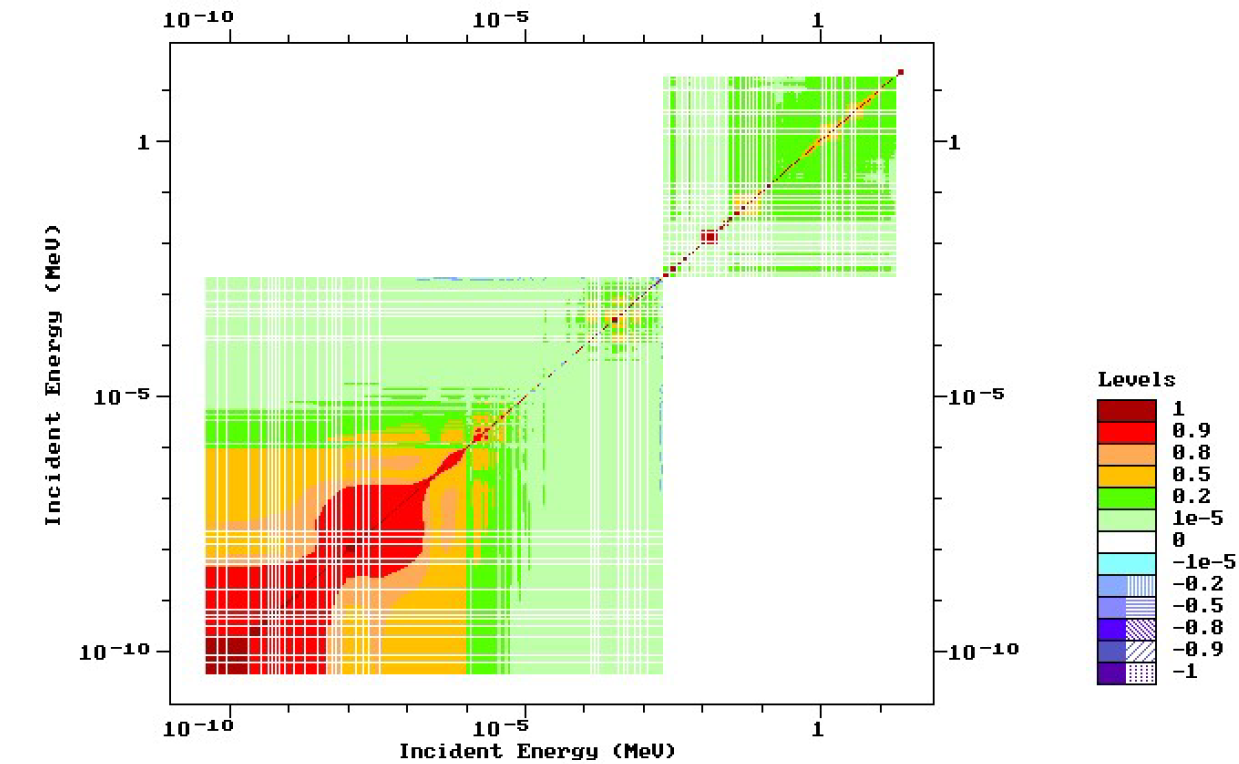
\includegraphics[width=\linewidth]{Figures/Chapter2/U235_nf_coor.png}
	\caption[$\mathrm{^{235}}$U (n,f) correlation matrix.]{$\mathrm{^{235}}$U (n,f) correlation matrix\cite{ENDF}.}
	\label{fig:coor}
\end{figure}

\ Integral experiments are extremely dependent on the underlying reactions that make up the net result. 
Therefore, there are generally larger variances in the the reactions that are part of the total cross-section. 
Figure \ref{fig:U235rel} displays the relative uncertainty of the $\mathrm{^{235}}$U (n,f) cross-section compared to the total cross-section. 
Figure \ref{fig:Bi209rel} displays the relative uncertainty of the total cross-section of $\mathrm{^{209}}$Bi compared to the (n,2n) reaction cross-section. 

\begin{figure}[htb!]
	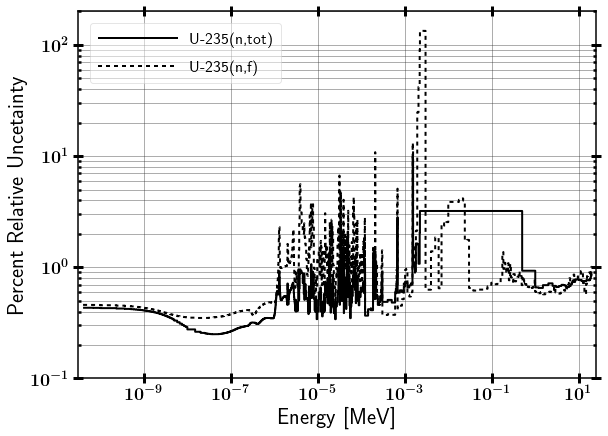
\includegraphics[width=0.9\linewidth]{Figures/Chapter2/U235_RelUncert.png}
	\caption[Percent relative uncertainty in $\mathrm{^{235}}$U (n,f) cross-section compared to $\mathrm{^{235}}$U (n,tot) cross-section]{Percent relative uncertainty in $\mathbf{^{235}}$U (n,f) cross-section compared to $\mathbf{^{235}}U$ (n,tot) cross-sections \cite{ENDF}.}
	\label{fig:U235rel}
\end{figure}

\begin{figure}[htb!]
	\includegraphics[width=0.9\linewidth]{Figures/Chapter2/Bi_209_RelUncert.png}
	\caption[Percent relative uncertainty in $\mathrm{^{209}}$Bi (n,2n) cross-section compared to $\mathrm{^{209}}$Bi (n,tot) cross-sections]{Percent relative uncertainty in $\mathbf{^{209}}$Bi (n,2n) cross-section compared to $\mathbf{^{209}}$Bi (n,tot) cross-sections \cite{ENDF}.}
	\label{fig:Bi209rel}
\end{figure}

\ The uncertainty in $\mathrm{^{235}}$U (n,f)  and $\mathrm{^{209}}$Bi highlight a couple key attributes relevant to nuclear data. 
First, the component reactions that make up the total cross-section almost always have a higher relative uncertainty because integral cross-section experiments can more accurately be measured through attenuation of a ``beam" of neutrons. 
The underlying reactions are generally more difficult to characterize. 
Second, the $\mathrm{^{235}}$U (n,f) cross-section relative uncertainty near 2.2 keV is 133.6\%. 
This large uncertainty implies that the cross-section must go negative to capture the full distribution of possible total cross-sections within a given confidence interval when utilizing a Gaussian distribution.
This suggests that the confidence intervals are not symmetric and points to utilizing alternative functional forms for the cross-section probability distribution functions. 
% Have you seen anything that would indicate the uncertainties assigned are not assuming a gaussian distribution? 
% Yes somewhat. I know all of the codes sample from a multivariate normal distribution, but:
% From ENDF - It is not necessary to assume that the density functions are normal in shape,
% or otherwise, unless one must estimate the probability that the true value lies within a certain
% range of the expected value.
This is obviously non-physical; however, it gives scope to the magnitude of the uncertainty in the underlying cross-sections over difficult experimental energy ranges. 
Next, the $\mathrm{^{235}}$U reactions are more thoroughly studied as compared to $\mathrm{^{209}}$Bi. 
Over the majority of the energy range, The uncertainty in the $\mathrm{^{235}}$U cross-section is below one percent relative error, largely driven down by thermal nuclear reactor experiments, while $\mathrm{^{209}}$Bi cross-section has a larger error around 5\%. 
Finally, areas where the cross-sections are low have representative larger relative errors; this is the case near the threshold of the $\mathrm{^{209}}$Bi (n,2n) reaction as shown in Figure \ref{fig:Bi209rel}. 

\subsection{Nuclear Data Stochastic Sampling}

\ The two primary methods that exist for uncertainty quantification of radiation transport simulations are linear perturbation and stochastic sampling Monte Carlo approaches \cite{Rochman2011}. 
First order linear perturbation theory is not always adequate for large uncertainties or incorporating second order effects from the uncertainty in the neutron transport; however, it does have broad uses in the reactor community.
Stochastic sampling has grown in popularity as computational resources have improved. 
Stochastic methods rely on performing independent neutron transport calculations with perturbed nuclear data libraries sampled based on the covariance of the cross-sections using the multivariate normal distribution to build a distribution of responses \cite{Aures2017}. 
The generalized multivariate normal distribution is a function of the nuclear cross-section mean values ($\boldsymbol{\mu}$), length \textit{k}, random solution vector ($\boldsymbol{X}$), covariance matrix ($\boldsymbol{\Lambda}$) is given by

\begin{equation} \label{eq:Cov4}
f(\boldsymbol{X}) = \dfrac{exp(-0.5(\mathbf{X}-\boldsymbol{\mu})^{T}\mathbf{\Lambda}^{-1}(\mathbf{X}-\boldsymbol{\mu}))}{\sqrt{(2\pi)^{k}\mid \mathbf{\Lambda} \mid}}.
\end{equation}

\noindent Several Monte Carlo sampling methods have been created to capture the effect of nuclear data covariance on nuclear engineering problems, including SCALE Sampler, NUSS, and SHARK-X \cite{Diez2015, Zhu2015a, SCALE, Aures2017}.  

\ Deficiencies with the stochastic sampling approach are generally associated with the nuclear data libraries and the sampling method. 
First, nuclear data uncertainty is often above 100\% in energy regions where a measurements do not exist, so the value of the cross-section is not well characterized. 
Second, the nuclear data uncertainty is assumed to be normally distributed; however, alternative forms may be more appropriate. 
In stochastic sampling approaches, these two factors lead to truncation of large uncertainties to prevent performing neutron transport calculations with negative cross-sections. 
Although negative cross-sections are non-physical, the truncation may underestimate the calculated uncertainty which can have an effect if the experiment is performed in these energy domains when using the Gaussian distribution. 
Finally, component cross-sections which make up the total cross-section are constrained to sum to the total cross-section. 


\section{Monte Carlo Neutron Transport}
\subsection{Monte Carlo Neutron Transport Theory}
\ Monte Carlo methods for neutron transport leverage pseudo-random sampling, nuclear data, and material specifications to build a simulation of the particle transport in space, direction, energy, and time \cite{Luciano2012a}. 
Neutron interactions are sampled with probability distribution functions (PDFs) for aspects such as path length traveled and interaction type \cite{Lewis1984}. 

\ An objective of a neutron transport calculation is to determine the average behavior of particles with-in the system. 
This can be captured with the volume averaged scalar flux, $\bar{\phi_V}$, defined as

\begin{equation} \label{eq:flux}
\bar{\phi_V} = \frac{1}{V}\int_V dV \int_t dt \int_E dE\: \phi(\vec{r}, E,t),
\end{equation}

\noindent where  $\bar{\phi_V}$ is given as a function of energy ($E$), position ($\vec{r}$) and time ($t$).
Monte Carlo methods approximate the scalar flux with either track length or collision estimates \cite{Lewis1984}. The track length estimator is 

\begin{equation} \label{eq:track}
\bar{\phi_V}  = \frac{W \: T_l}{V \: N},
\end{equation}

\noindent where the path length score for the flux is based on the distance traveled ($T_{l}$) and is normalized by the particle weight (W), cell volume (V), and number of histories sampled (N).

\ Statistics often drive the uncertainty in a Monte Carlo simulation as systematic uncertainties are generally not considered due to computational costs. 
The ``true" mean value, $\mu$, of a response PDF is the expectation value, $E(x)$, which is estimated with a sample mean, $\bar{x}$. 
According to the Central Limit Theorem, the sample mean approaches the real mean as the number of samples, $N$, goes to infinity, and the distribution of sampled $x_i$ follows a Normal distribution.
The sample mean can be calculated as

\begin{equation} \label{eq:sampmean}
\bar{x} = \frac{1}{N}\sum_{i=1}^N x_i. 
\end{equation}

\noindent Therefore, sample variance, ($S_x^2$) can be computed as

\begin{equation} \label{eq:sampvar1}
S_x^2 = \frac{1}{N-1}\sum_{i=1}^N (x_i - \bar{x})^2,
\end{equation}

\noindent and the variance of the mean, ($S_{\bar{x}}^2$), is simply

\begin{equation} \label{eq:sampvar}
S_{\bar{x}}^2 = \frac{S_x^2}{N}, 
\end{equation}

\noindent where $S_x^2$ is defined with the sample variance.  
Therefore, the statistical uncertainty in the results decreases with $\sqrt{N}$. 
The precision of the result can be improved with more histories, shrinking the spread in $x_i$. 
However, the accuracy cannot be improved. 
Accuracy is impacted by systematic errors, such as uncertainty in the nuclear data.

\subsection{Comparison of Monte Carlo Neutron Transport Results}\label{'secMC'}

The results from different Monte Carlo simulation codes often produce slightly different results. The outputs are generally in better agreement for criticality calculations of critical assemblies and nuclear reactor analysis. 
It is important to gauge the effect of utilizing different transport codes to see how much variance is expected. 
Some of the differences that effect Monte Carlo simulations are within the structure of the code itself, statistical error, or different starting seeds, while others are based on the nuclear data that may be altered, geometry or source implementation, or user error.

Criticality is a well-understood nuclear engineering problem that the nuclear data libraries are validated against. 
Wang, \textit{et al.} conducted on a high temperature pebble-bed reactor compared SCALE's CSAS6 module for criticality calculations to MCNP5's kcode\cite{Wang2014}. 
The results showed a difference for calculating $k_{eff}$ to be on the order 0.5\%. 
% Should this be 10^4? Everything I have says 10^5, and wiki
This variance can easily be handled for reactor operations; however, this highlights that even well understood problems do have differences based on simulation code. 
A similar study conducted by Johnson \textit{et al.} of a pebble-bed reactor determined that the difference in $k_{eff}$ in MCNP to SCALE was near half a percent  \cite{Johnson2007}. %With a varied geometry? Yes, they looked at a bunch of configurations to optimize it. I'm taking that out now, it was confusing wording  on my end. --- For what output? keff? 
In another study, Chen \textit{et al.} compared the average gamma-ray dose outside of a spent nuclear fuel cask \cite{Chen2011}. 
The dose rates predicted by SCALE and MCNP simulations varied as much as 27\%. 
Again, this shows that the less benchmarked studies can have large code-to-code disagreements. 

\section{Foil Activation}
\subsection{Foil Activation Theory}

Foil activation is a method of characterizing an incident neutron flux through unfolding the response of the foils using the energy-dependent nuclear reaction channels in the foil. 
Activation experiments are essential for testing that requires small geometries or where electronic equipment used in measuring techniques will be damaged. 

Activation foils produce measurable radioactive isotopes during the course of irradiation. 
The production rate of radioactive isotopes is negated by radioactive decay processes, which place an upper limit on the radioactivity of a foil \cite{Knoll}. 
The saturated activity 

\begin{equation} \label{eq:InfReactionRate}
A_{\infty} = R = \int_{E1}^{E2} \phi(E) \Sigma(E) _{act} V
\end{equation}

\noindent is equivalent to the reaction rate ($R$), which is a function of the energy dependent flux ($\phi$), the macroscopic reaction activation cross-section ($\Sigma(E)_{rxn}$), and the volume of  the foil ($V$). The energy term ($E1$) is zero in many cases; however, threshold reactions require the incident neutron to be of higher energy to enable the reaction channel. 

When six half-lives have elapsed, a foil will have reached approximately 98\% of its saturation activity, neglecting spatial and energy self-shielding effects \cite{Knoll}. 
When the activation is not sufficient to fully saturate the foil, a correction needs to be made.
The activation of the foil for a given irradiation time ($t_{i})$ is given as 

\begin{equation} \label{eq:ReactionRate}
A_{0} = A_{\infty}(1-e^{-\lambda t_{i}}), 
\end{equation}

\noindent where $\lambda$ is of the decay constant of the radioactive product.

The formula can be simplified in the limit of irradiation times much less than 
the half-life of the activation products. In this case, the production rate is 
much larger than the decay from radiation, so the rate of production of the 
radioisotope is driven only by the reaction rate. The neutron pulse length at the NIF is on the order of shakes (1 shake = 10 nanoseconds), while the reaction channels of interest have half-lives on the order of an hour or longer. Therefore this approximation can be made for the foil activation. The time integrated flux, or neutron fluence ($\Phi$), can be used to determine the total reactions, ($R_{total}$),
over an irradiation period, given by

\begin{equation} \label{eq:NIFrxnRate}
R_{total} = \int_{E1}^{E2} \Phi(E) \Sigma(E) _{act} V \:dE.
\end{equation}

% I've tried to make the use of () or ,, for the definition of symbols consistent, but you may want to double check.
Experimental measurements of the activity must be corrected to deduce the original activity of the foil ($A_{0}$) immediately after irradiation as shown in Equation \ref{eq:MeasActivity}. 
The activity is corrected for the radioactive decay occurring between the end of irradiation and the start of counting ($t_{d}$). 
A similar correction factor based on the count time ($t_{c}$) provides a correction for radioactive decay during counting that can result in a reduction of counting rates by the end of the counting period. 
Additionally, the detector efficiency for the given gamma-ray energy ($\epsilon$) and relative gamma intensity ($I_{\gamma}$) must be taken into account. 
The gamma intensity may also include a branching ratio if applicable to the decay mechanism.
Finally, the measured counts ($C$) is reduced by the background counts ($B$). 
All corrections included, less self-shielding effects, provide a formulation for converting counts to post-irradiation activity as  

\begin{equation} \label{eq:MeasActivity}
A_{0} = \frac{\lambda (C-B) e^{\lambda t_{d}}}{\epsilon (1-e^{-\lambda 
t_{c}})I_{\gamma}}.
\end{equation}


\subsection{Selection of Experimental Foils}\label{FoilsHere}
\ The method of foil activation has been studied in-depth in the 
nuclear sciences and engineering community. A list of the various 
requirements that are of importance for a neutron activation foil experiment 
with neutron energies in the range of thermal to approximately 20 MeV are summarized below\cite{Knoll,Luciano2012a,Kuijpers1977}.

\begin{itemize}
	\item The reaction neutron cross-section is extremely important for foil 
	activation, and there are a few key parameters that should be considered. 
	First, the magnitude of the cross-section determines the 
	reaction rate of the product nuclides. A large cross-section allows for 
	more activation, and therefore, better results when analyzing the activation 
	foils. Second, the uniqueness of the cross-section shape is used to unfold 
	the incident neutron energy spectrum. An (n,$\gamma$) cross-section may 
	peak in a particular region, which is essential to providing information of the 
	neutron flux in that energy region. Alternatively, a threshold reaction, 
	such as an (n,2n), is important for providing information about the flux at 
	higher energies. Third, activation of the selected foils for an experiment should cover  
	the entire energy range of the incident neutron flux. Finally, the cross-section
	must be well characterized with low uncertainty over the neutron energy range of
	interest.   
    
    \item The range of activation product half-lives applicable for a particular experiment depends on availability of detectors and the time before counting the foils post-irradiation. A long lived radioisotope 
    will be available for counting for longer times at the expense of the total activity. The opposite is true for short 
    half-lives. Half-lives on the order of an hour to a few years are generally used; however, the half-life must also be balanced with the 
    production of the radioisotope to understand the entire picture. 
    
    \item The elemental, isotopic, and chemical purity of the activation foil should be 
    well known. An unknown composition foil can produce erroneous 
    results. 
    
    \item Interfering reaction channels and decay emissions should be avoided. 
    An example of this is natural copper, which has multiple 511 keV emissions 
    from different reaction channels. It is difficult to distinguish these 
    gamma-rays to determine activation in counting. Similar problems arise in 
    multi-isotope materials that have multiple reactions producing the same 
    nuclide. For example, the $\mathrm{^{106}Cd}$ (n,$\gamma$) reaction produces the same 
    isotope as a $\mathrm{^{108}Cd}$ (n,2n) reaction, which complicates spectral unfolding. 

    \item The activation foil should be optically thin to not cause 
    perturbations of the neutron flux.
    An additional benefit of relatively thin foils is that the gamma-ray emissions for detection are not significantly attenuated through self-shielding. 
    In general, adding additional foils helps to improve the unfolding 
    results, as long as the entire foil set remains generally optically thin \cite{Vagena2018b}. 

    \item The decay nature of the product nuclide should preferably be a gamma-ray emitter. 
    Gamma-ray detection can provide fine energy resolution to 
    determine activation. 
    The discrete gamma-ray emissions provide a means of determining the source and magnitude of the the foil activation. 
    The energy of the gamma is also of importance. 
    Semiconductor detection methods have a peak intrinsic efficiency near 100 keV with some variance depending on whether the semiconductor is p-type or n-type. 
    Beta spectroscopy is also a potential option that may be considered; however, the resolution is not as good as gamma spectroscopy.  
\end{itemize}

\section{Neutron Energy Spectrum Unfolding}

Foil activation experiments are a well-documented method for determining an incident neutron energy spectrum \cite{Knoll}. 
The foils are irradiated under a nearly equivalent neutron flux, which serves to activate the foil samples through nuclear reaction channels, each of which has a unique response 
function with respect to the neutron flux. 
The nuclear data and activities of the foils can be used to unfold the incident neutron energy spectrum.

In an ideal situation, the number of foil reactions ($i$) would be selected based on the number of energy groups ($j$) required, and the problem would be formulated as \cite{Vagena2018b, Luciano2012a}  

\begin{equation} \label{eq:BadWaytoGetFlux}
    A_{i}= \sum_{j=1}^{N} \; \Sigma_{i}(E_{j}) \;\Phi(E_{j}) \;V,\;\; 
    i=1..m.
\end{equation}

\noindent In practice, this formulation of the unfolding problem is not used as it often provides nonphysical results.
The issue is caused by the varying shapes of reaction cross-sections, which create a poorly constructed matrix and a limit on the number of foils that can be used at a time to prevent changing the neutron flux. 
There are many methods that aim to provide solutions to the generally degenerate neutron spectrum. 

A few examples of unfolding methods include  matrix inversion, least-squares spectral adjustment, and stochastic algorithms\cite{Reginatto2010}. 
Direct matrix inversion was previously discussed in the setup of the unfolding problem. 
Matrix inversion is generally seen as ``ill-posed" and can lead to non-physical results, such as negative fluxes \cite{Reginatto2010, Vagena2018b}. 
Stochastic methods rely on random sampling to derive a best-fit or average over a group of reasonably well-fitting spectra\cite{Reginatto2010}. 
The least-squares method minimizes the chi-square based on a guess spectrum, activation information, and nuclear data \cite{Perey1977}.
The least-squares method is also known as spectral adjustment and can incorporate more information, most notably the underlying energy dependent nuclear data, into the determination of the resultant spectrum \cite{Perey1977}.  

The general formulation of the least-squares method is derived in this case by minimizing the error between activation results to the nuclear data convolved with the guess neutron spectrum \cite{Perey1977}. 
The chi-square ($\chi^{2}$) is given as per degrees of freedom ($\nu$) as a function of the uncertainty, activation rates $A_{i}$, nuclear data, and measured results. 
The $\chi^{2}$ formulation of the least-squares approach can be reduced if there is no time dependence of the neutron flux as

\begin{equation} \label{eq:LeastSq2}
\dfrac{\chi^2}{\nu}= \dfrac{1}{\nu}\sum_{i=1}^{m} \; \dfrac{(\sum_{j=1}^{N} \Sigma_{i}(E_{j}) \;\Phi(E_{j})-\dfrac{A_{i}}{V_{Foil}})^{2}}{\sigma_{i}^{2}} \,\;\;.
\end{equation}

Providing an initial spectrum is generally required for the unfolding methods. 
The activities produced for the foils is often highly degenerate, where an infinite number of spectra could provide the same observable end-point. 
The initial spectrum allows for the insertion of more physics-based results into the unfolding. 
For neutron spectra, an initial guess spectrum is often created with a particle transport code or a deterministic solution. 
Alternatively, an initial spectrum could be selected from published results \cite{VegaCarrillo2002}. 